% ==========================================================================
% SI Appendix for the PNAS-format version. Holds everything moved out of
% the 8-page article: the extended methods, the moved results detail and
% figures, and the full-length draft's supplementary sections. Numbers are
% the audited pack numbers (docs/paper-pack/data).
% ==========================================================================
\documentclass[11pt]{article}
\usepackage[T1]{fontenc}
\usepackage[utf8]{inputenc}
\usepackage{lmodern}
\usepackage[a4paper,margin=2.5cm]{geometry}
\usepackage{graphicx}
\usepackage{booktabs}
\usepackage{longtable}
\usepackage{amsmath}
\usepackage{caption}
\usepackage[numbers,sort&compress]{natbib}
\usepackage[hidelinks]{hyperref}
\usepackage{url}
\usepackage{float}
\newcommand{\doi}[1]{doi:~\href{https://doi.org/#1}{\nolinkurl{#1}}}
\graphicspath{{../figures/main/}{../figures/appendix/}{../figures/appendix/cities/}}
\captionsetup{font=small,labelfont=bf}
\newcommand{\gref}{g(15)}
\newcommand{\pw}[1]{$p_{\mathrm{wild}} = #1$}
\newcommand{\pperm}[1]{$p_{\mathrm{perm}} = #1$}
\renewcommand{\thesection}{S\arabic{section}}
\renewcommand{\thetable}{S\arabic{table}}
\renewcommand{\thefigure}{S\arabic{figure}}

\title{\textbf{SI Appendix}\\[4pt]\large Two geographies of urban deprivation:
everyday services and emergency care across European cities}
\author{Tina Comes}
\date{}

\begin{document}
\maketitle
\tableofcontents
\clearpage

% ==========================================================================
\section{Extended Materials and Methods}\label{si:methods}
% ==========================================================================

\subsection{Two meanings of unreachable}
Unreachable conflates two situations that the pipeline keeps apart. A
cell with no network path reaches zero facilities of any service in any
mode; it is detected once by a service- and mode-independent probe, so the
everyday and emergency masks are equal by construction, and it enters no
statistic. A cell that is routable but has no facility of a given service
within that service's cut-off is service-deprived rather than unreachable:
it receives a large finite effective time (the routing cut-off) so that
the everyday level saturates and the cell stays on the map. Merging the
two would let one sparse service mask a whole city. Travel-time summaries
(mean, median, 90th percentile) are computed over reachable cells only and
reported beside the unreachable population share.

\subsection{Congestion and substitutability in the everyday regime}
For each everyday service the two-step floating catchment area factor
computes the supply-to-demand ratio of each facility,
$R_j = S_j / \sum_i P_i K(t_{ij})$ with a Gaussian kernel $K$, and
converts it into a time inflation $c_j = (R_{\mathrm{ref}}/R_j)^{\gamma}$
relative to the demand-weighted median ratio of the city. The soft
minimum over reachable facilities lies between the nearest adjusted time
and that time less $\ln(n)/\kappa$. The everyday composite is the
weighted mean of the per-service levels over the categories reachable
from the cell; school and green-space sub-types share one extraction and
weigh 0.5 each so that each of the five categories counts once. Because
network walking time scales inversely with speed, the 3.5\,km/h often
assumed for elderly and mobility-impaired residents is equivalent to
lowering $t_0$ from 15 to about 11 minutes at the baseline speed, which
the 10-minute variant of the sensitivity grid covers.

\subsection{Anchor structure of the emergency cost}
The 8-minute mark cannot play the half-maximum role the 15-minute
inflection plays for the everyday level: convexity caps $g(8)/g(15)$ at
0.427 given $g(4)/g(15) = 0.10$, so the anchor structures of the two
regimes are genuinely different. Free-flow civilian drive times anchor the
cost scale and are not response-time predictions: dispatch and turnout are
unmodelled, lights-and-siren travel is faster than civilian flow, and
free-flow understates congested cores relative to the periphery.

\subsection{Vulnerability strata}
Vulnerability is analysed on two strictly separated levels. The
census-harmonised age strata (top quartile of the share under 15, of the
share aged 65 and over) exist for every city and are pooled. National
fine-grid strata (lowest rent and ownership quartiles, finer age cuts)
exist only where a national grid does, use different definitions, and are
reported per city and never pooled. Each stratum is compared against the
cells on which its own variable is published, because national grids are
published where the population is large enough and that is not a random
subset of a metropolitan area. Within-stratum inequality uses the
concentration index \citep{wagstaff1991measurement}.

\subsection{Clustering and coverage grades}
The city vector (means, Ginis, coupling, compounding, tail shares,
within-city density slopes, log population) is robust-scaled, with the
zero-inflated tail shares opened by $\log(1+x)$, and clustered by k-means
and Ward with $k$ selected by silhouette over 2--6
\citep{rousseeuw1987silhouettes}. Every partition carries a bootstrap
adjusted Rand index over resampled cities \citep{hubert1985comparing}, a
Gaussian silhouette null (same-covariance multivariate-normal draws pushed
through the same selection) and the ARI against the region partition. When
the winning split isolates an outlier group below a quarter of the sample,
a peeled second pass re-scales and re-clusters the remaining cities with
the same diagnostics. Desert is the main pass's outlier group, partial
desert the peeled pass's smaller cluster, covered the rest. A feature-set
check re-runs the whole procedure with the 8- and 15-minute benchmark
shares added. The graded scaling model regresses log emergency cost on
centred log population, grade dummies and their interaction with
country-clustered errors.

\subsection{Deprivation against access}
Every headline size regression is re-run on the deprivation-free
travel-time indicators (median, mean and, for the emergency regime, the
90th-percentile minutes); the deprivation-based and time-based Gini
families are correlated across cities; the desert capitals' ratios to the
sample are computed under both measures. The everyday 90th percentile is
not regressed because above the walking cut-off the everyday composite
time behaves as a count of unmet service categories rather than a travel
time.

\subsection{Robustness harness}
A structured, non-probabilistic sweep recomputes the rank-based targets
over a defensible envelope. Layer 1 varies curvature within the fixed
forms. Layer 2 swaps the forms while pinning the same anchors: a concave
Box-Cox everyday level through the same half-maximum and ceiling, and for
the emergency regime an exponential escalation
\citep{holguinveras2013objective} and a bounded survival-based curve, both
solved from the 8- and 15-minute anchors so that the three emergency forms
coincide inside the benchmark window and diverge only beyond it. Layer 3
sweeps the accessibility model (soft-minimum $\kappa$, congestion exponent
$\gamma$, catchment bandwidth, number of nearest facilities, everyday mode
set, unreachable fill, off-network policy) from the saved travel-time
matrices. A threshold axis sweeps the typology cut from the 40th to the
75th percentile.

\subsection{Reproducibility}
The pipeline is configuration-driven with provenance sidecars on every
derived travel-time matrix, and no deprivation parameter is hard-coded.
Every number quoted in the article is checked against its source table by
an automated audit of 190 checks run in continuous integration; the
main-text figures are drawn from the pack tables and the configuration by
scripts in the study repository.

% ==========================================================================
\section{Deprivation vs access: exact values}\label{si:depvsaccess}
% ==========================================================================

\begin{table}[H]
\centering
\caption{Size elasticities of deprivation-based and minutes-based
outcomes (log-log, country-clustered SEs, 67 cities), plotted in main-text
Fig.~2A. Source: \texttt{deprivation\_vs\_access.csv}.}
\label{tab:si-depvsaccess}
\small
\begin{tabular}{@{}llrrr@{}}
\toprule
Regime & Outcome & Elasticity & $p$ & $R^2$ \\
\midrule
Everyday  & mean deprivation level      & $-0.196$ & $<0.001$ & 0.44 \\
Everyday  & median walk time            & $-0.237$ & $<0.001$ & 0.16 \\
Everyday  & mean walk time              & $-0.178$ & $<0.001$ & 0.31 \\
\addlinespace
Emergency & mean deprivation cost       & $-0.059$ & 0.16     & 0.02 \\
Emergency & median drive time           & $-0.043$ & 0.09     & 0.04 \\
Emergency & mean drive time             & $-0.043$ & 0.05     & 0.04 \\
Emergency & p90 drive time              & $-0.059$ & 0.02     & 0.05 \\
\bottomrule
\end{tabular}
\end{table}

\begin{table}[H]
\centering
\caption{The five emergency-desert capitals: median drive time to the
nearest emergency facility and its ratio to the 67-city sample median
(12 min) against mean emergency deprivation cost (multiples of \gref{})
and its ratio to the sample value (1.14). Source:
\texttt{desert\_access\_contrast.csv}.}
\label{tab:deserts}
\small
\begin{tabular}{@{}lcrrrr@{}}
\toprule
City & Country & Median time (min) & Time ratio & Mean cost & Cost ratio \\
\midrule
Vilnius        & LT & 14.0 & 1.17 & 5.39 & 4.72 \\
Ljubljana      & SI & 23.0 & 1.92 & 4.96 & 4.34 \\
R\={\i}ga      & LV & 13.5 & 1.13 & 3.37 & 2.95 \\
Bucure\c{s}ti  & RO &  8.5 & 0.71 & 3.21 & 2.81 \\
Tallinn        & EE & 13.0 & 1.08 & 2.80 & 2.45 \\
\bottomrule
\end{tabular}
\end{table}

% ==========================================================================
\section{Size regressions: diagnostics and the conditional emergency Gini}\label{si:scaling}
% ==========================================================================

The everyday elasticity of $-0.196$ is stable under country fixed effects
($-0.17$), leave-one-out city deletion (envelope $-0.204$ to $-0.185$,
Athina the most influential city), outlier-robust estimators (Huber
$-0.196$, median regression $-0.223$) and exclusion of the five desert
capitals ($-0.203$). Equivalence at the stricter $\pm 0.10$ bound is not
shown for the emergency elasticity, hence ``bounded within $\pm 0.13$''.

The emergency-Gini size behaviour is conditional on the beyond-benchmark
escalation form. Under the bounded survival-based curve the Gini is
size-flat ($+0.001$, $p = 0.97$); under polynomial Box-Cox escalation, the
published baseline, it is size-flat across the whole curvature sweep
($-0.006$ to $+0.014$, none significant), in agreement with the
deprivation-free travel-time Gini ($-0.015$, $p = 0.42$); under exponential
escalation it rises ($+0.098$, $p = 0.0003$), because exponential pricing
turns the Gini into an index of extreme-tail depth (it saturates at a
median of 0.96, decouples from the time distribution's inequality,
$\rho = 0.04$, and tracks the beyond-45-minute population share,
$\rho = 0.45$), and how many minutes past the cut-off the worst-served
residents sit does grow with size even though the tail's population share
does not (beyond-30-minute share elasticity $-0.003$, $p = 0.99$).

\begin{figure}[H]
\centering
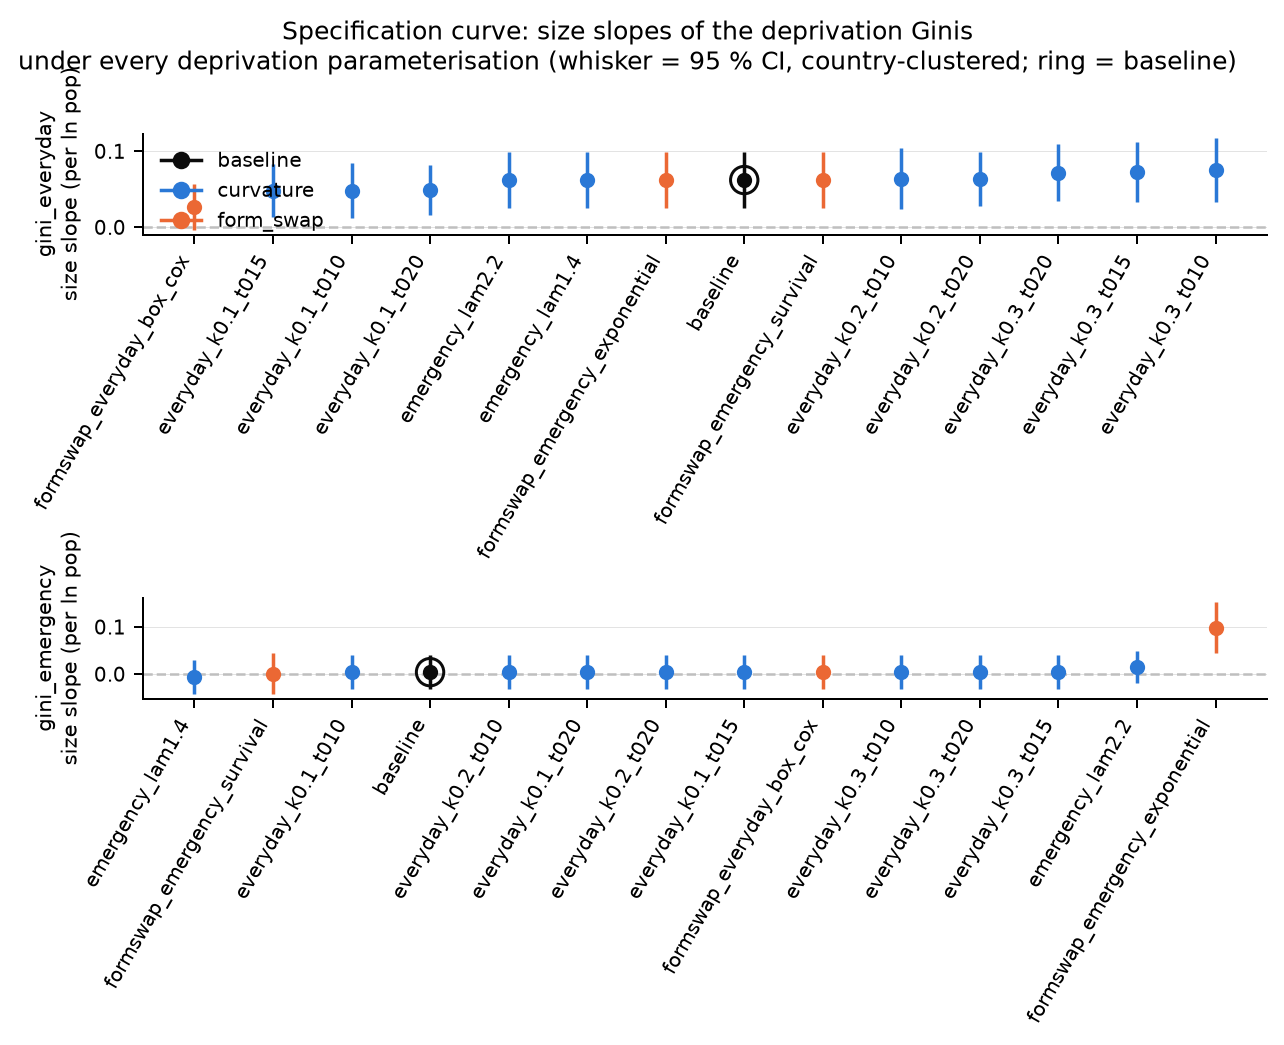
\includegraphics[width=.95\textwidth]{specification_curve.png}
\caption{Specification curve of the inequality-scaling slopes. Top:
everyday Gini; bottom: emergency Gini. Each point is the size elasticity
of the within-city Gini re-estimated under the ringed baseline or one of
the 14 alternative deprivation parameterisations (blue: curvature grid;
orange: functional-form swaps); whiskers are country-clustered 95\,\%
CIs. The everyday-Gini slope is positive under every specification
($+0.026$ to $+0.075$; significant in 13/14, the exception the concave
Box-Cox form swap at $p = 0.083$). The emergency-Gini slope splits by
beyond-cut-off escalation form.}
\label{fig:si-speccurve}
\end{figure}

\subsection{Additional robustness of the size regressions}\label{si:scaling-extra}
Table~\ref{tab:si-scaling-extra} re-estimates the four headline size
regressions with further checks. Residual spatial dependence is absent
for the everyday level (Moran's $I = 0.06$, permutation $p = 0.41$) and
present for the emergency level ($I = 0.23$, $p = 0.0015$) and for both
Ginis ($I = 0.20$ and $0.39$): cities close to one another share what size
does not explain, which is the country and coverage structure of
Section~\ref{si:regional}. The slope estimates are unaffected; inference
is country-clustered throughout and regional contrasts permute countries,
so the dependence enters the tests at the level at which it arises.
Adding mapped GP density per 100k inhabitants as a control leaves the
everyday elasticity at $-0.185$ (wild $p = 0.0002$) and the everyday-Gini
elasticity at $+0.051$ ($p = 0.0006$); the control is significant in both
everyday equations and in neither emergency equation. A centred quadratic
in log population is not significant for the everyday level or either
Gini and is significant for the emergency level ($-0.169$, wild
$p = 0.001$; $-0.104$, $p = 0.010$ with coverage-grade dummies): the
size-stratum means of the emergency deprivation cost are 1.15, 1.69, 1.56
and 0.70 multiples of \gref{} from the smallest to the largest stratum, an
inverted U in which the middle strata, where the desert and
partial-desert cities sit, carry the highest cost and the four FUAs above
five million the lowest. With identical regressors in both regime
equations, joint estimation coincides with equation-by-equation OLS; the
residual correlation it would add is $r = 0.51$ for the means and
$r = 0.19$ for the Ginis ($p = 0.13$). The minimum detectable emergency
elasticity at 80\,\% power is 0.12.

\input{tables/scaling_extra}
\input{tables/scaling_crossequation}

% ==========================================================================
\section{Regional structure}\label{si:regional}\phantomsection\label{sec:coverage}
% ==========================================================================

\begin{figure}[H]
\centering
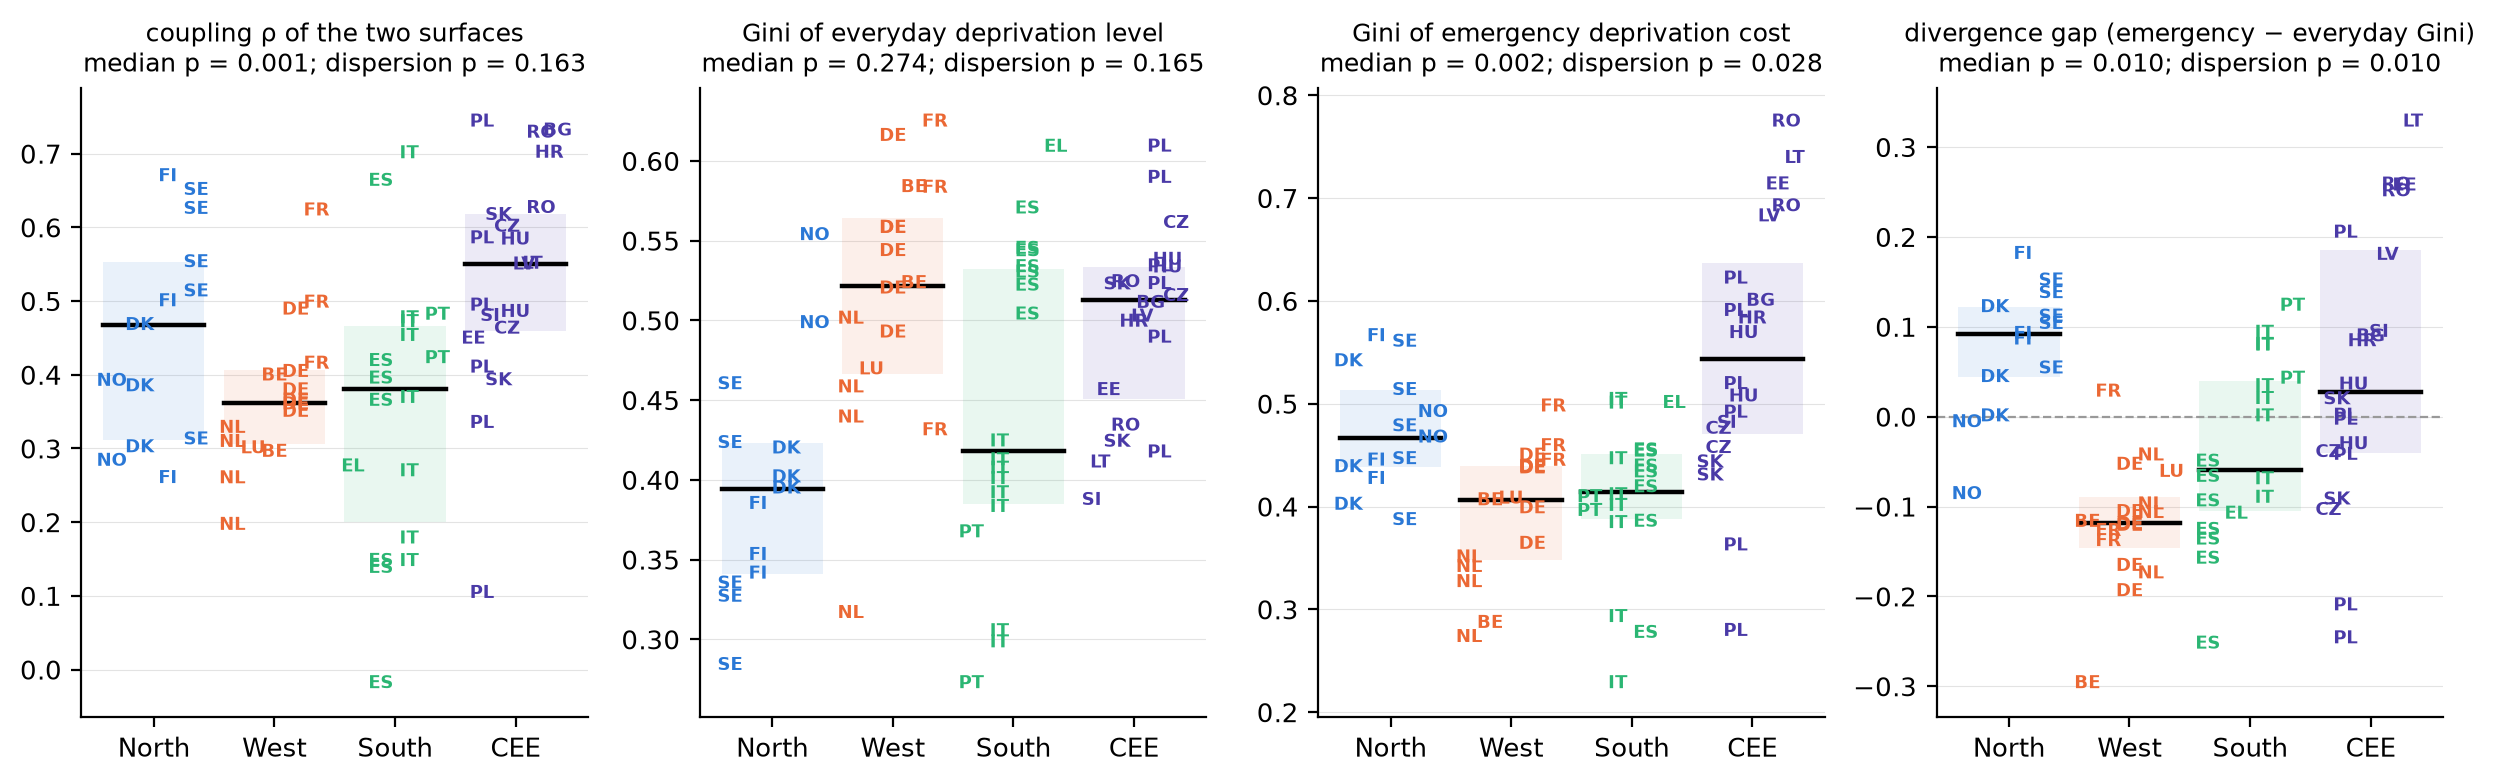
\includegraphics[width=\textwidth]{region_strips.png}
\caption{Regional structure of the divergence, each city drawn as its
country code (bar: regional median; band: interquartile range) for the
coupling $\rho$, the everyday Gini, the emergency Gini and the divergence
gap. Panel titles give the country-permutation p-value of the regional
contrast in medians and in dispersion. The everyday-Gini panel shows the
Spanish and Greek cities above the Italian and Portuguese ones with no
overlap, which is why that contrast is a country contrast and is not
claimed regionally.}
\label{fig:si-regions}
\end{figure}

The West's inequality problem is everyday-side (median divergence gap
$-0.12$); the North's is emergency-side ($+0.09$). The everyday Gini's
apparent regional contrast has a city-level ANOVA $p = 0.0007$ and a
country-permutation $p = 0.27$; half of its variance lies between
countries within regions, more than for any other indicator. It coincides
with the general-practitioner tagging artefact: the median FUA has 10.8
mapped GPs per 100k inhabitants, but the country medians are 2.1 in
Sweden, 2.3 in Portugal, 2.6 in Finland and 3.5 in Italy against 24.5
across the West, because primary care there sits in health centres
OpenStreetMap tags differently, which overstates everyday deprivation
levels and compresses their within-city spread. Mapped GP density is
uncorrelated with city size (log-log slope $+0.09$, country-clustered
$p = 0.29$). Eight cities have only one of the two emergency services
mapped (Athina, Br\u{a}ila, Helsinki, Lahti, Norrk\"oping, Szeged,
Talavera de la Reina, \v{Z}ilina); the composite renormalises weights over
the services present, their median mean emergency cost is 0.197 against
0.169 for the rest, and none is in the desert group.

\begin{figure}[H]
\centering
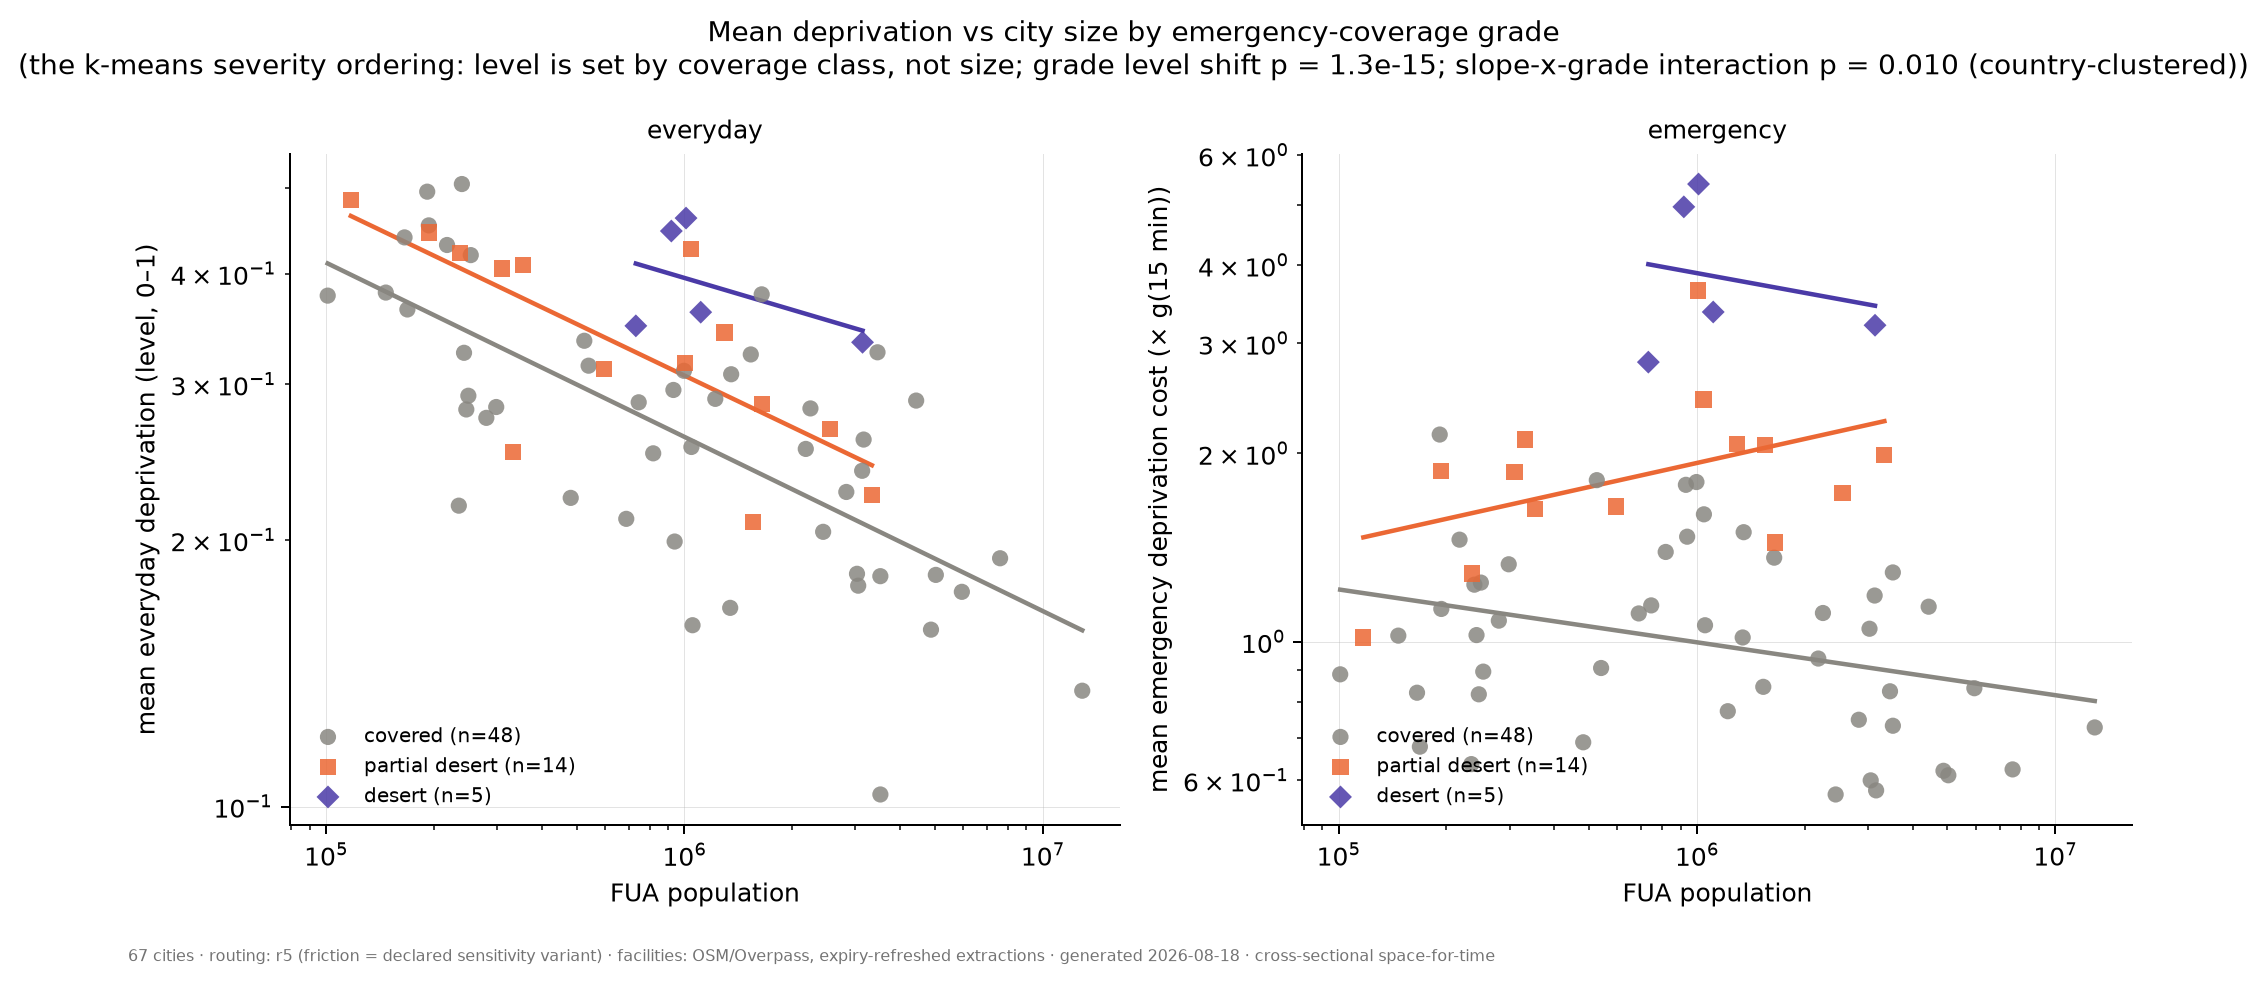
\includegraphics[width=.95\textwidth]{scaling_by_coverage_grade.png}
\caption{Mean deprivation against city size by emergency-coverage grade,
per regime (left: everyday level; right: emergency cost). The grade shifts
the emergency level (country-clustered Wald $p \approx 1.3\times10^{-15}$;
median 1.02 / 1.87 / 3.37); the slope-by-grade interaction is $p = 0.010$
under the current 48/14/5 grades but $p = 0.17$ under the pre-refresh
50/12/5 grades, so it is boundary-sensitive and not headlined. The
boundary cities are Br\u{a}ila and \L{}om\.za. Within-grade fits are plain
OLS over few cities.}
\label{fig:si-grade}
\end{figure}

\input{tables/regional_variance}
\input{tables/regional_dispersion}
\input{tables/regional_no_deserts}
\input{tables/grade_by_region}
\input{tables/south_split}

\begin{figure}[H]
\centering
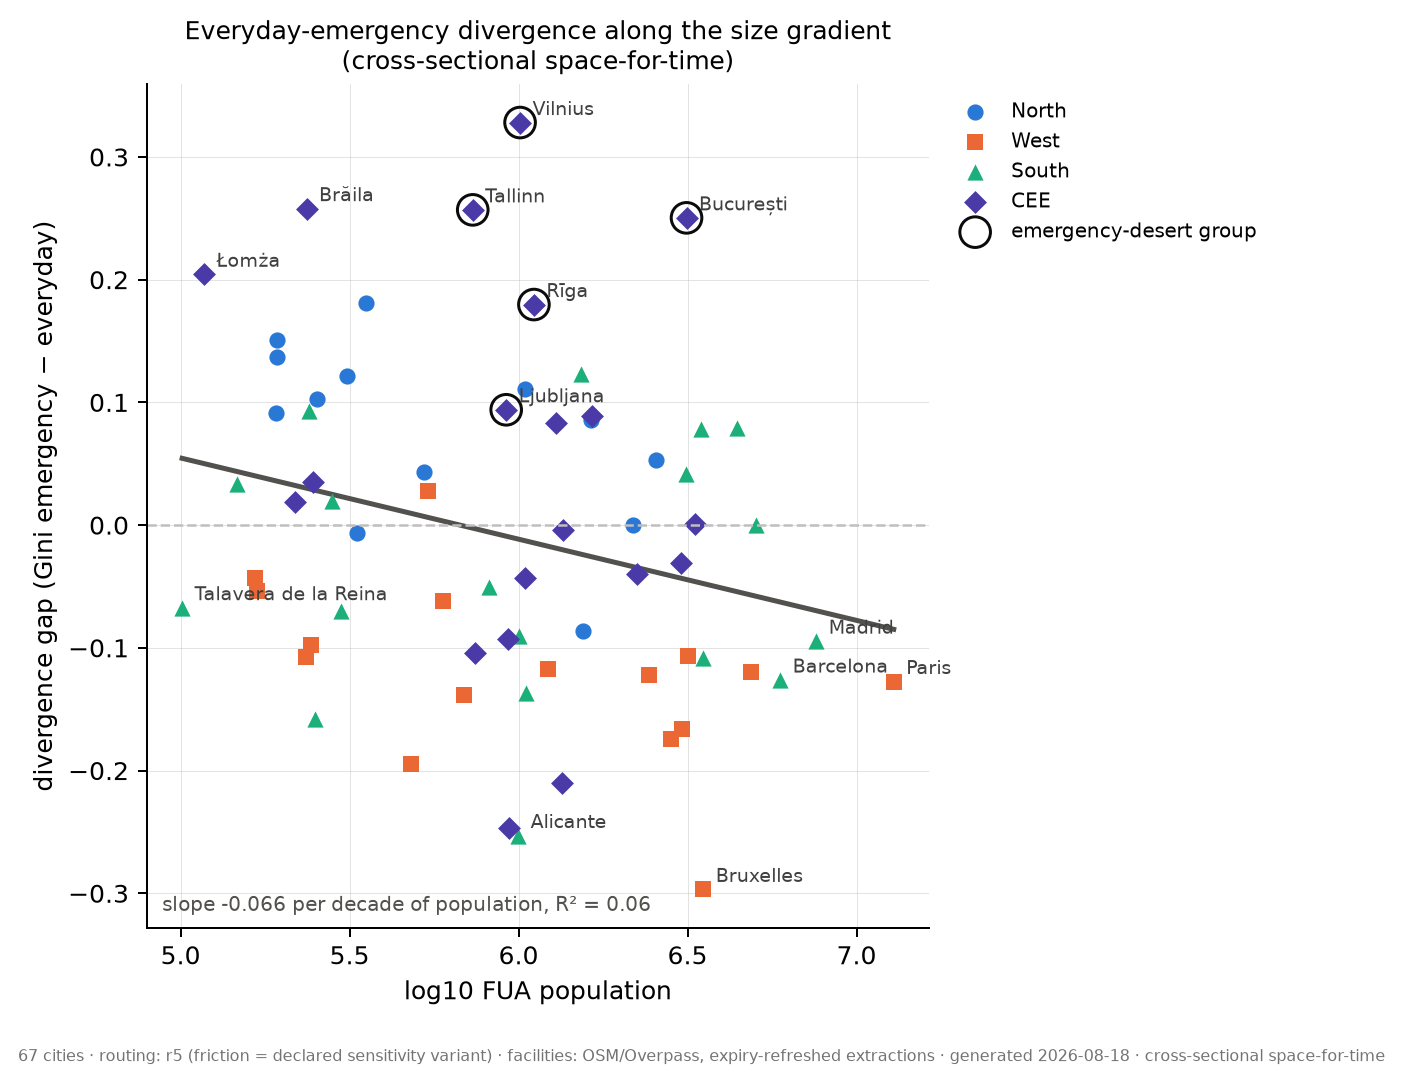
\includegraphics[width=.85\textwidth]{size_gradient.png}
\caption{The divergence gap (emergency Gini minus everyday Gini) against
$\log_{10}$ FUA population. The gap falls weakly with size ($-0.066$ per
decade, $p = 0.012$, $R^2 = 0.06$); the coupling $\rho$ ($p = 0.14$) and
the compounding share ($p = 0.06$) show no significant size gradient.}
\label{fig:si-sizegradient}
\end{figure}

% ==========================================================================
\section{Compounding: coupling, threshold sensitivity and spatial anatomy}\label{si:compounding}
% ==========================================================================

The ``how high is high'' percentile cut moves the HH share by 29.8
percentage points at the median city, against 1.4 under the whole
deprivation-curvature grid and 0.9 under the functional-form swaps. The
continuous compounding intensity has fixed anchors (1/3 under
independence, 1/2 under perfect coupling, 1/4 under perfect divergence)
and differs regionally (\pperm{0.0023}, strongest in Central-Eastern
Europe). Maps are read under two rules: legends carry population-weighted
shares while the picture is area-weighted, and no single cell's class is a
finding, since roughly 24\,\% of population flips class between routing
engines.

\begin{figure}[H]
\centering
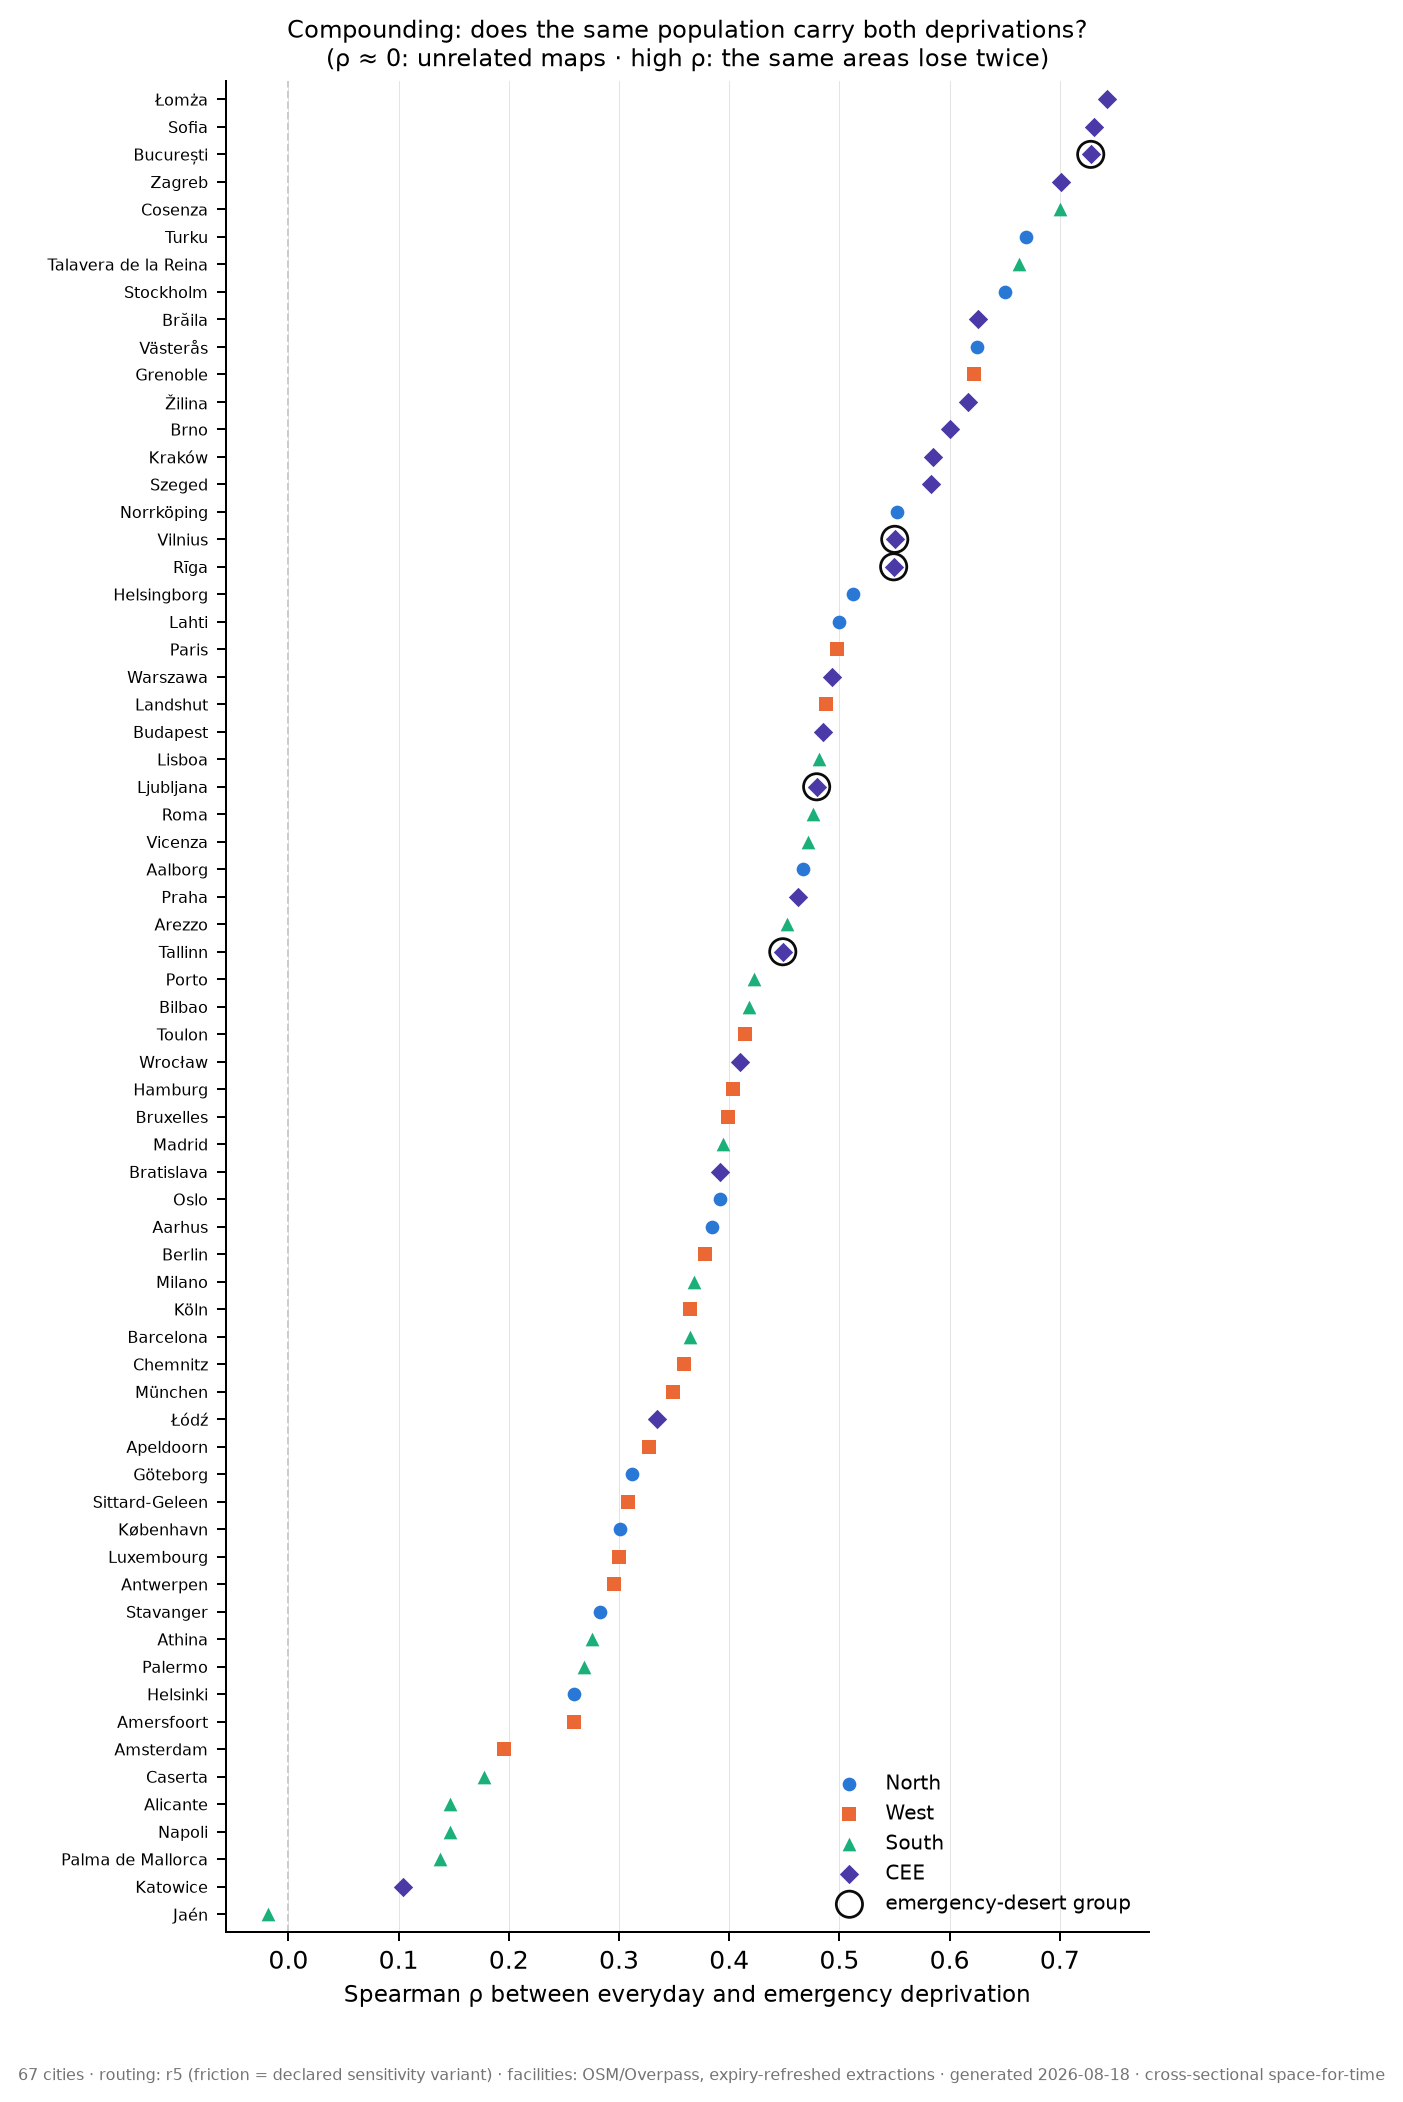
\includegraphics[width=.9\textwidth]{rho_ranked.png}
\caption{Coupling of the two deprivation surfaces across the 67 cities:
Spearman $\rho$ between the everyday and emergency percentile surfaces,
cities ranked ($-0.02$ to $0.74$). Colours mark macro-regions; the
emergency-desert capitals are outlined. The HH share exceeds the 25\,\%
independence benchmark in 66 of 67 cities (mean 33\,\%).}
\label{fig:si-rho}
\end{figure}

\begin{figure}[H]
\centering
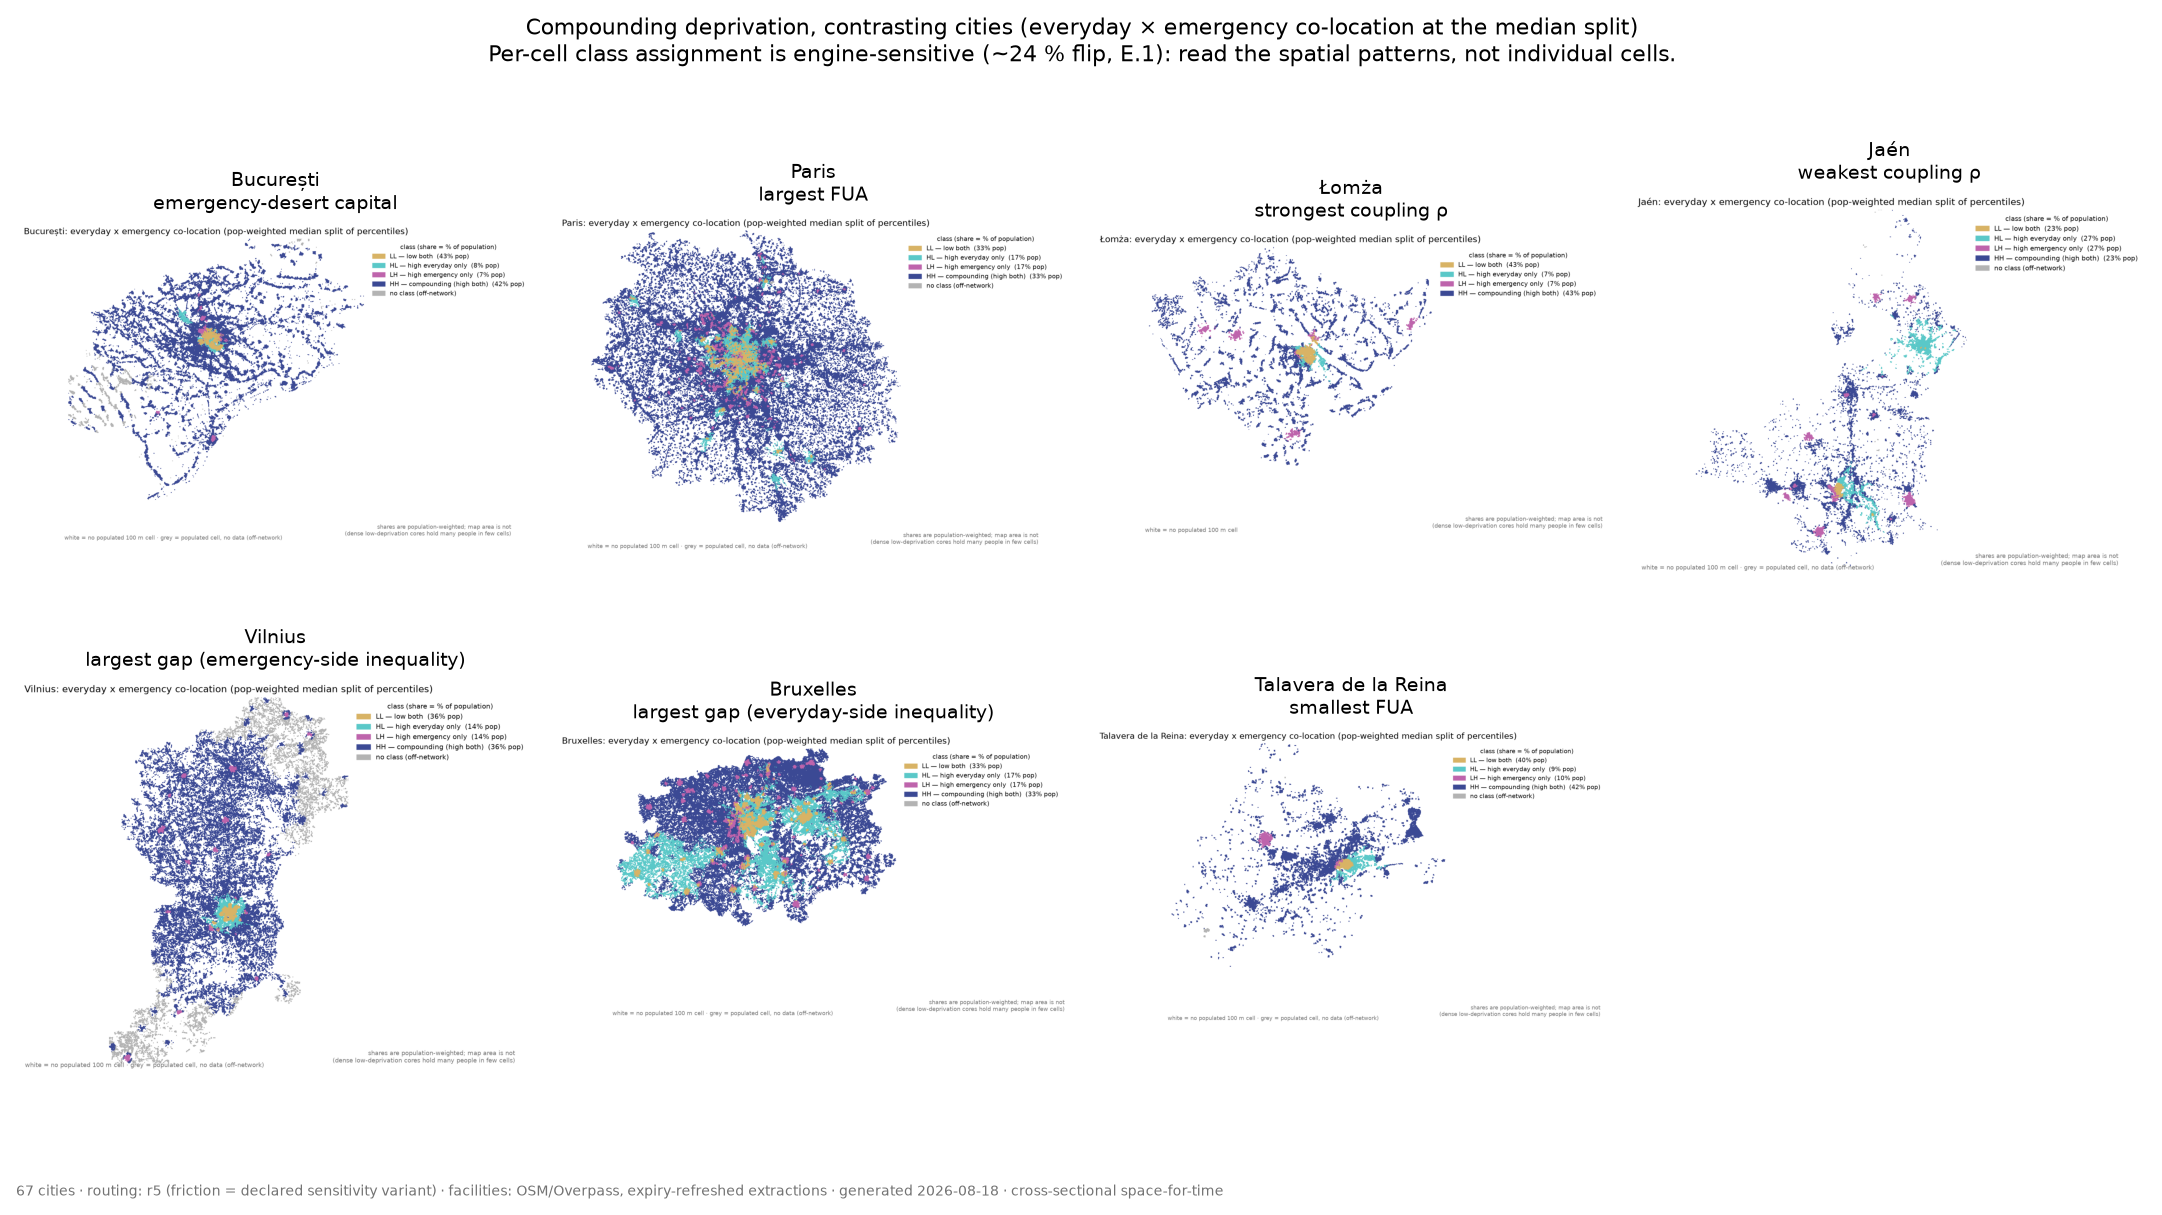
\includegraphics[width=\textwidth]{compounding_gallery.png}
\caption{Compounding gallery: median-split co-location typology for
contrasting cities (all 67 maps in Section~\ref{si:gallery}). Colours: LL
both low, HL high everyday only, LH high emergency only, HH compounding.
Legend shares are population-weighted; the maps are area-weighted.}
\label{fig:si-gallery}
\end{figure}

% ==========================================================================
\section{Robustness of the deprivation layer}\label{si:robustness}
% ==========================================================================

What is varied is drawn in main-text Fig.~1: the Layer-1 curvature grid
($k \in \{0.1, 0.2, 0.3\}$ per minute $\times$ $t_0 \in \{10, 15, 20\}$
minutes for the everyday logistic; $\lambda \in \{1.4, 1.8, 2.2\}$ for the
emergency Box-Cox) and the Layer-2 form swaps calibrated to the same
anchors. How far the results move is in Table~\ref{tab:envelopes}. Levels
are not robust, and are not meant to be: curvature alone moves a typical
city's everyday Gini by 0.24 Gini points, which is why the calibration
carries information and why every slope claim is defended by the
specification curve. Ranks and classes are robust: the same grid moves the
compounding share by 1.4 percentage points at the median, the form swaps
by 0.9, against 29.8 for the threshold. City-level Gini orderings survive
with two scoped exceptions: rank agreement with the baseline stays at
$\rho \geq 0.90$ over the curvature grid and the everyday form swap, while
both emergency escalation swaps reorder the emergency-Gini ranking
(exponential $\rho = 0.19$; bounded survival $\rho = 0.49$) because each
changes what that Gini measures. Deprivation-variant flip cells average
18.1\,\% of city population (range 5.2--53.0\,\%), with the HH class share
moving 2.1 percentage points on average and 6.1 at most. The clustering
survives its feature-set choice (main partition ARI 1.00, peeled 0.97).
The routing-engine cross-check bounds the engine's leverage: switching
engines moves travel-time levels by 34--314\,\% and flips the class of
roughly 24\,\% of population per city, while aggregate class shares move
at most 0.7 percentage points.

\begin{table}[H]
\centering
\caption{Sensitivity envelopes: median min--max envelope width across the
67 cities per sweep axis and target. The form-swap emergency-Gini
envelope spans the three beyond-cut-off escalation hypotheses. Source:
\texttt{deprivation\_sensitivity\_summary.csv}.}
\label{tab:envelopes}
\small
\begin{tabular}{@{}lrrr@{}}
\toprule
Sweep axis & Everyday Gini & Emergency Gini & HH share \\
\midrule
Curvature (Layer 1)            & 0.244 & 0.170 & 0.014 \\
Form swap (Layer 2)            & 0.035 & 0.649 & 0.009 \\
``How high is high'' threshold & --    & --    & 0.298 \\
\bottomrule
\end{tabular}
\end{table}

\begin{figure}[H]
\centering
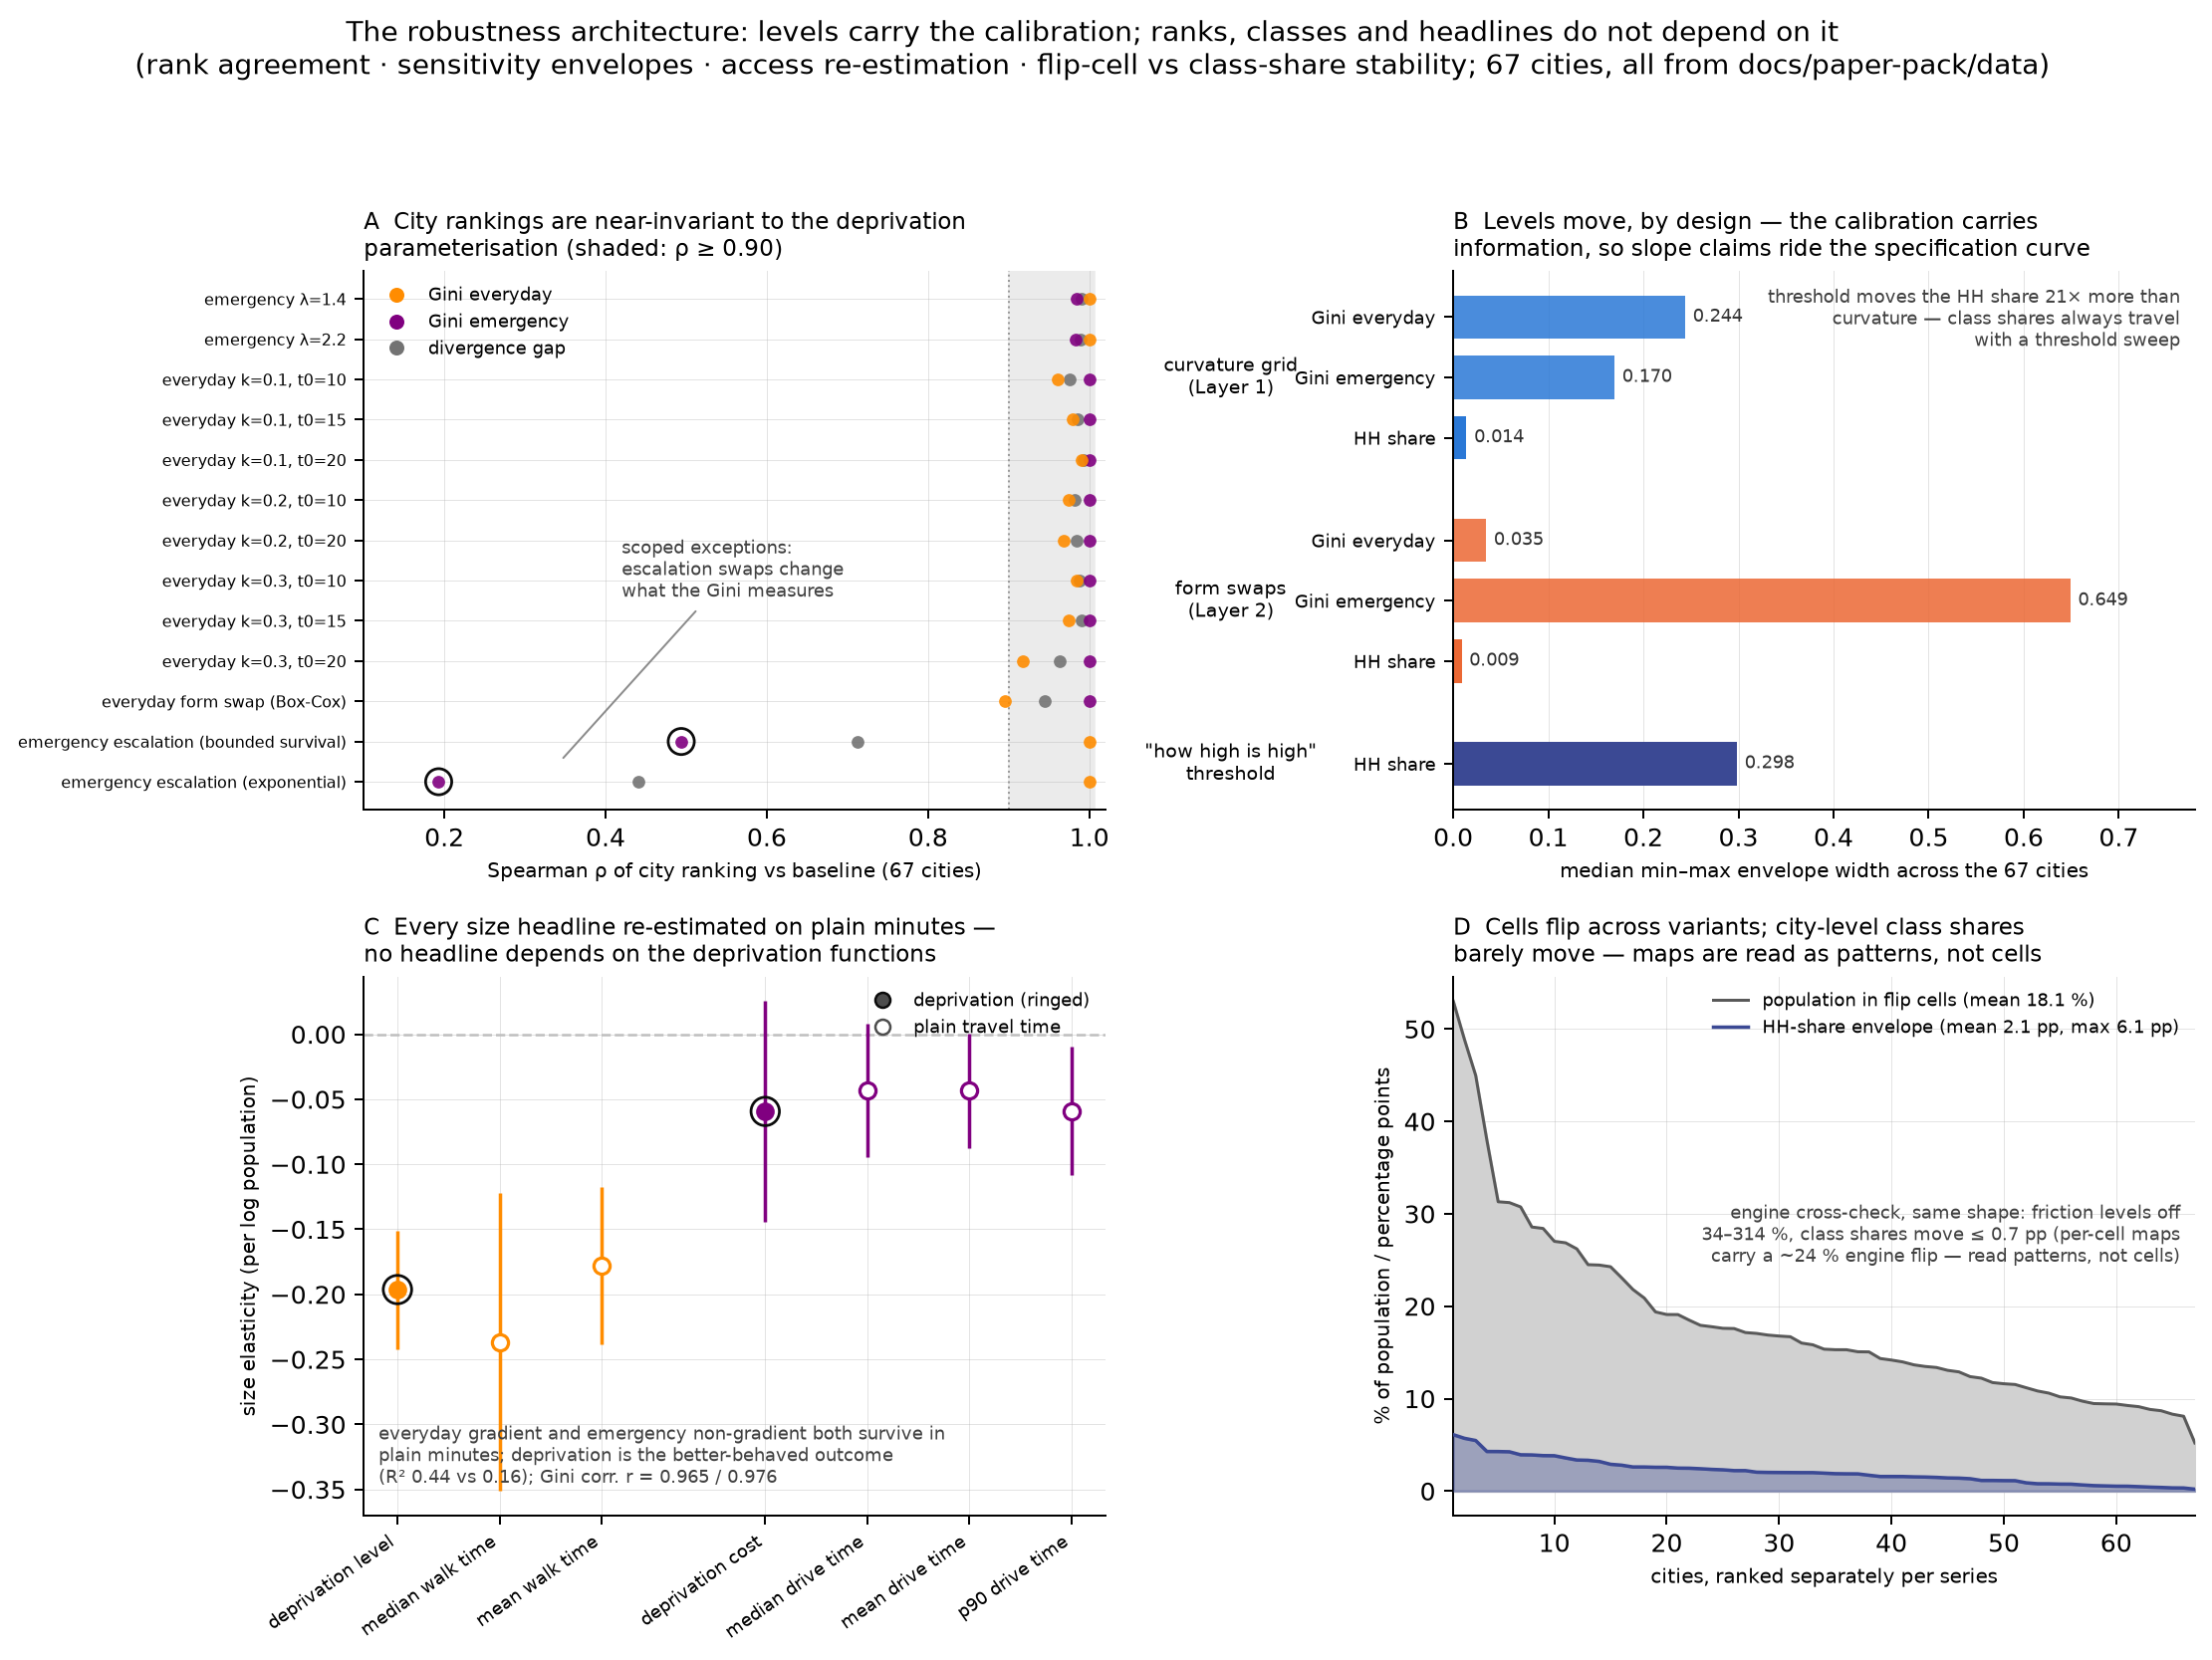
\includegraphics[width=\textwidth]{robustness_architecture.png}
\caption{The robustness architecture in one view: rank agreement across
deprivation variants, envelope widths per axis, access-based
re-estimation of every headline, and flip-cell against class-share
stability, with the routing-engine cross-check alongside.}
\label{fig:si-architecture}
\end{figure}

% ==========================================================================
\section{Validation exercises}\label{si:validation}
% ==========================================================================

\paragraph{Routing-engine cross-check.} Re-running Hamburg and K\"oln under
the friction-surface engine against the R5 baseline shows travel-time
levels understated by 34--314\,\% with city-specific Gini bias (emergency
Gini $-30$\,\% in Hamburg, $-18.5$\,\% in K\"oln), which demoted friction
to a sensitivity variant. Aggregate typology class shares move $\leq 0.7$
pp and the coupling $\rho$ by $\leq 11\,\%$, while roughly 24\,\% of
population flips per-cell class.

\paragraph{OpenStreetMap completeness.} Benchmark against national
registries where available: Germany, pharmacies ratio 0.976, hospitals
1.24 (the hospital ratio carries a verify-before-publication flag). The
per-city facility counts provide the cross-country completeness picture
and surface the GP tagging artefact.

\paragraph{External benchmark.} The German INKAR accessibility indicators
reproduce the study's German pharmacy and supermarket access patterns; no
comparable emergency-side benchmark is available.

\paragraph{Re-anchor verification.} The emergency reporting anchor moved
from $g(45)$ to $\gref$ in August 2026. For the three cities re-seeded
from stored artifacts every rank-based indicator is identical to machine
precision and the level ratio equals $g(45)/g(15) = 6.7307$ to
$10^{-15}$; the other 64 cities were byte-identical between the two runs.

% ==========================================================================
\section{Indicator glossary}\label{si:glossary}
% ==========================================================================

\begin{table}[H]
\centering
\caption{Compact glossary of the indicators used in the article.}
\small
\begin{tabular}{@{}p{0.32\textwidth}p{0.62\textwidth}@{}}
\toprule
Term & Meaning \\
\midrule
FUA & Functional urban area (Eurostat/OECD): city plus commuting zone; the unit ``city''. \\
Everyday regime & Five walkable service categories (GP, pharmacy, supermarket, school, green space); deprivation is a bounded \emph{level} in $[0,1]$. \\
Emergency regime & ED hospital and ambulance station, reached by car; deprivation is an unbounded convex \emph{cost} in multiples of \gref{}. \\
$\bar D_{\mathrm{ev}}$, $\bar C_{\mathrm{em}}$ & Population-weighted mean deprivation per regime; scales are incomparable across regimes. \\
$G_{\mathrm{ev}}$, $G_{\mathrm{em}}$ & Population-weighted within-city Gini of each surface. \\
Divergence gap & $G_{\mathrm{em}} - G_{\mathrm{ev}}$; positive = emergency-side inequality problem. \\
$\rho$ & Spearman correlation of the two population-weighted percentile surfaces. \\
LL/LH/HL/HH & Median-split co-location classes; HH = compounding; independence = 25\,\%. \\
Compounding intensity & Population-weighted mean of $\min$(everyday pct, emergency pct); 1/3 independence, 1/2 coupled, 1/4 divergent. \\
Coverage grade & Severity ordering from the two clustering passes: covered / partial desert / desert. \\
Elasticity & Slope of log outcome on log population (space-for-time). \\
Wild cluster bootstrap & Country-clustered resampling; the citable p for scaling claims. \\
$p_{\mathrm{perm}}$ & Permutation p-value reshuffling whole countries across macro-regions. \\
TOST & Two one-sided equivalence tests; positive evidence a slope lies within a bound. \\
Specification curve & Headline regression re-estimated under every deprivation parameterisation. \\
Flip cells & Cells whose typology class changes under any deprivation variant. \\
\bottomrule
\end{tabular}
\end{table}

\clearpage
% ==========================================================================
\section{Per-city table}\label{si:cities}
% ==========================================================================
\input{tables/cities_descriptives}

\clearpage
% ==========================================================================
\section{Per-city compounding maps}\label{si:gallery}
% ==========================================================================
The median-split co-location typology map of each of the 67 cities,
ordered by population. Legends carry population-weighted class shares;
the maps are area-weighted. Read for spatial pattern only.

\input{tables/city_gallery}

\bibliographystyle{unsrtnat}
\bibliography{../references}
\end{document}
